\documentclass[a4paper,10pt]{article}
\usepackage[utf8]{inputenc}
\usepackage{url}
\usepackage{graphicx}

%opening
\title{Parallel sorting combining Quicksort and Mergesort algorithms}
\author{Santiago Munín González}

\begin{document}

\maketitle
\clearpage
\begin{abstract}
  This article describes an application which uses both Quicksort\footnote{\url{http://en.wikipedia.org/wiki/Quicksort}} and Mergesort\footnote{\url{http://en.wikipedia.org/wiki/Merge_sort}} algorithms 
  with multiple processes in order to increase the performance (execution time) of the common problem of sorting a set of numbers.
  
  The multiple processes are organized as a binary tree with different levels (from 0 to $\log_2 nproc$), 
  beign $nproc$ the number of involved processes. Each process will sort their subarray using Quicksort, and, in the next levels of the tree,
  some of them will merge it with the sorted subarray of another process. This operation will be repeated until the first process has the whole sorted array. 
  
  This solution decreases the execution time and allows a larger number of elements to be sorted if we execute this application 
  in more than one computer (because it could avoid memory overflows when computing a huge number of elements).
  
  About the tools, this program was written in Java and uses the FastMPJ\footnote{\url{http://fastmpj.com/}} library in order to implement the communication between the processes and 
  JUnit\footnote{\url{http://www.junit.org/}} (unit testing framework).
  
\end{abstract}
\clearpage

\section{Design and implementation}
  This section will describe all the problems I had to face during the development process and its solutions. Also, it will describe the basic architecture of
  processes and how they communicate between themselves.
  
  The basic operations used are two: sort a subarray (with the Quicksort algorithm) and merge two sorted arrays into a new sorted array 
  which contains both of them.
  
  \subsection{Processes distribution and communications flow}
    The main problem was how to manage to do all the merges quickly and taking advantage of all the involved processes.
    Steps:
    
    \begin{itemize}
     \item 1. Each process receives its subarray and sortes it.
     \item 2. The $numberOfProcesses$ sorted arrays have to be merged into $numberOfProcesses / 2$.
     \item 3. Keep merging until the parent process has the whole initial array (now sorted).
    \end{itemize}
    
    Each merge requires half of the previous processes, so it can be organized as follows:
\hspace{1.5cm}
    \begin{figure}[h]
  \begin{center}
  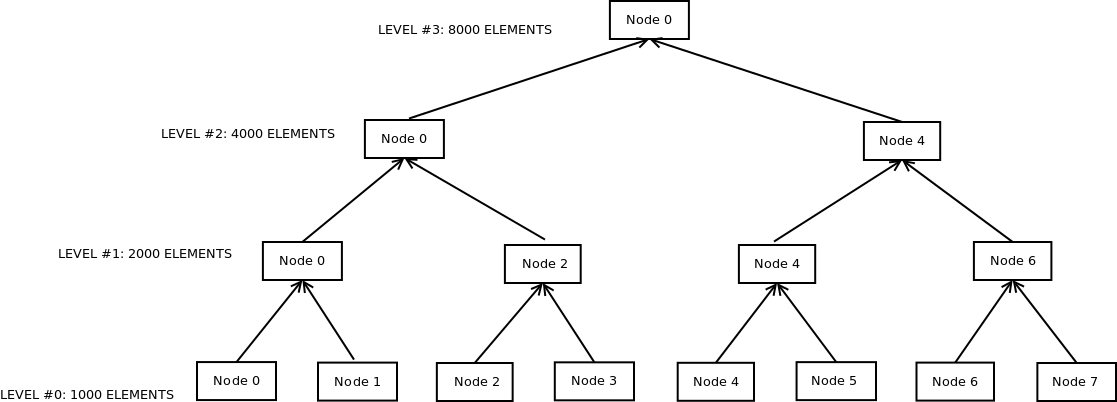
\includegraphics[scale=0.35]{sorting_tree.png}
  \caption{Sorting tree}
  \end{center}
  \label{sortingTree}
\end{figure}
\hspace{1.5cm}
      
    Each level of the tree regards to an iteration, starting from the bottom. Once a process has sorted its array, it has to determine whether it has to send it to other process or receive another process' sorted array.
   \begin{itemize}
            \item If it has to send the array, it must calculate which the destination is. 
            
            $Destination = processId\ \&\ \neg(1 << height)$ $\rightarrow$ This turns off the appropriate bit to get the process id of the parent node. The parameter $height$ refers to the height of the node within the sorting tree.
            \item If it has to receive another one, it must calculate which process has sent it. 
            $Source = me\ |\ (1 << (height - 1))$ 
  \end{itemize}
    
  \subsection{Being aware of no longer needed processes}
  Regarding to the sorting tree (figure \ref{sortingTree}), there are processes which wouldn't have to keep working. In order to kill those processes, all of them check
   in each level of the sorting tree whether they have to work or not. If not, they just finish. Also, if the starting number of processes is not a power of two, 
   all remaining processes will just finish.
  
  \subsection{Class diagram}
  This program has a simple organization: A $ParallelSorter$ which uses some utilities which are offered by a couple of utilities classes.
  \begin{itemize}
   \item $ParallelSorter$: Main class, it just has to be instanced and call the $execute$ method.
   \item $ParallelUtils$: Contains all the FastMPJ code, wrapped in a more friendly set of methods.
   \item $SortUtils$: Contains some sort methods (like $merge$).
   \item $QuickSort$: It's a very good implementation of QuickSort, which allows to sort a high number of elements since it has a very good management of memory\footnote{This implementation isn't mine, it is freely avaliable here: http://www.augustana.ca/~mohrj/courses/2004.winter/csc310/source/QuickSort.mysoln.java.html}.
  \end{itemize}
  
  \subsection{Testing}
  The development process was supported by some unit tests over the $ParallelUtils$ and $SortUtils$ methods. Also, when the program finishes, 
  it always checks if the obtained solution is correct (checking if it has the same elements sorted in a non-decreasing way).

\section{Results}

  \subsection{Execution environment}
  \begin{itemize}
   \item {\bf CPU}: Intel i7-2670QM @ 2.20GHz (4 cores) with Hyper-threading
   \item {\bf Memory}: 8GB @ 1333MHz
  \end{itemize}

  \subsection{Measurements}
  Each combination of number of elements and processes were executed five times. In this table, the average time (in {\bf ms}) of each case was used to fill each cell. Also, you can 
  check the chart (figure~\ref{measurements}
  
  \begin{center}
\begin{tabular}{|l|l|l|l|l|}
\hline
& 1 process & 2 processes & 4 processes & 8 processes\\
\hline
$5*10^5$ elements & 70& 83.2 & 73.2 & 115.4\\
\hline
$5*10^6$ elements & 567.6 & 453.8 & 420 & 501.2\\
\hline
$5*10^7$ elements & 6246 & 4264 & 3344.6 & 3612.8\\
\hline
  \end{tabular}
  \end{center}
  
  \hspace{1.5cm}
    \begin{figure}[h]
  \begin{center}
  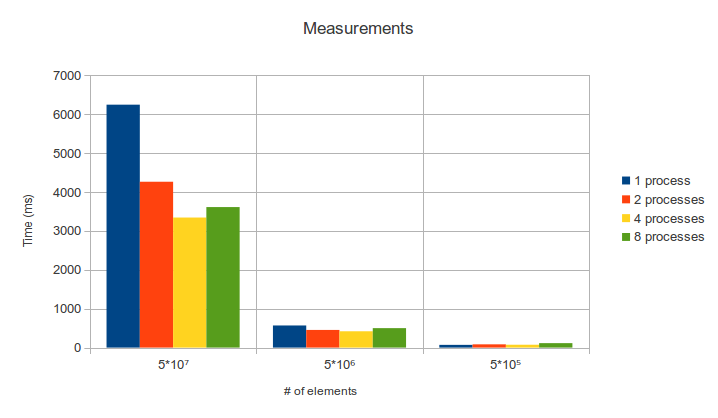
\includegraphics[scale=0.6]{measurements.png}
  \caption{Measurements}
  \end{center}
  \label{measurements}
\end{figure}
\hspace{1.5cm}

  \subsection{Conclusion}
  If the number of elements is high, incrementing the number of processes will improve the execution time. For example, when the number of elements were $5*10^7$, the program reached 
  a speedup of $6246/4264 = 1.8674$ (1 process vs 4 processes). However, there are two limitations where scaling the number of processes:
  \begin{itemize}
  \item Once the number of processes are more than the number of cores, part of the operations have to be done in sequential (since the CPU can't perform that number of operations simultaneously).
   \item As the number of processes increases, so does the ordering tree, and therefore the communications between processes. This is only worth it if the number of items is large, thus justifying the additional expense of communications. Notice that when the number of elements is $5*10^5$, the execution time increases with the number of processes. This is because is cheaper to sort that small number of elements 
    in a sequential way rather than in parallel (because the cost of the communications). This could be solved by improving the communications flow.
   
  \end{itemize}

\end{document}
